
\chapter{Analyse van de openstaande problemen}%Lars

% Analyse van de openstaande problemen, tekorten, eventuele foute beslissingen
\section{Tijdsduur backend API Calls}
\label{tijdsduur}
Zoals aangehaald in sectie \ref{sec: GCE} Google Cloud Endpoints is een van de nadelen van GCE de grote variatie in tijdsduur van backend API calls. Figuur \ref{fig:hist_getAllGroups} is een histogram die de relatieve frequentie weergeeft van de tijdsduur van een bepaalde API call; gelijkaardige histogrammen worden bekomen voor andere API calls. De histogram is gebaseerd op 26 meetpunten verspreid over 2 dagen. GCE houdt een bepaalde backend instantie niet continu in ingeladen op de servers. De grote variatie in de tijden is m.a.w. te wijten aan het opstarten van de instantie. Deze wachttijden hebben een negatieve impact op de gebruikerservaring. Indien de toepassing echter meer wordt gebruikt, is de backend instantie meer actief en vormen `koude missers' minder een probleem.
\begin{figure}[H]
	\centering
	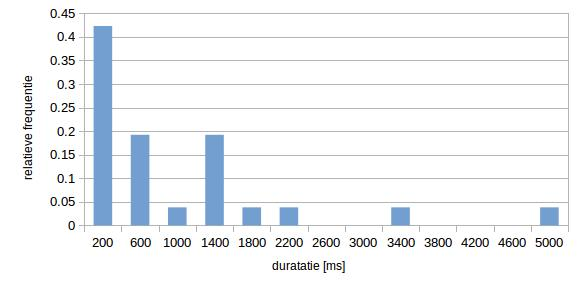
\includegraphics[scale=0.5]{prestatie_histogram_GCE}
	\caption{Histogram tijdsduur methode oproep getAllGroups()}
	\label{fig:hist_getAllGroups}
\end{figure}


\section{Checkin entiteiten}

In de huidige implementatie van de backend API wordt er voor iedere checkin van een gebruiker en voor iedere groep waartoe de gebruiker behoort een checkin entiteit aangemaakt. Hierdoor groeit het aantal entiteiten in de Checkin tabel zeer snel. Daarnaast komt nog dat Triump gebruik maakt van GAE Datastore voor de backend database. Bij het gebruik van deze Datastore horen quota's die beperkingen opleggen voor de grootte van de databank en voor het aantal entiteiten. 
% Hier moet een afbeelding komen:
% Grafiek van percentage types in datastore ...
De eenvoudigste oplossing voor dit probleem is het uitbreiden van de datastore door een dagelijks bedrag te betalen aan GAE. Een andere oplossing is het opstarten van een periodieke Cron job (zie sectie \ref{sec: GCE} Cron jobs) die bijvoorbeeld wekelijks de Checkin tabel `samenvat'. De samenvatting kan gebeuren door alle punten verzamelt door 1 groep op 1 locatie binnen een bepaalde periode toe te kennen aan 1 checkin entiteit. Op deze manier kan het aantal entiteiten drastisch beperkt worden. Nadeel van deze oplossing is het verlies aan informatie die mogelijks gebruikt kan worden voor het genereren van statistieken. 

Aangezien de opgelegde quota's m.b.t. de GAE Datastore ruimschoots voldoen en bijgevolg het probleem nog niet van toepassing is, zijn nog geen van beide oplossingen geïmplementeerd.
Indien het aantal gebruikers van Triump zou toenemen is het wel noodzakelijk een oplossing toe te passen.

\section{Android versies}

Android is een besturingssysteem waaraan continu wordt gesleuteld door Google. Er worden met regelmaat verbeteringen en wijzigingen doorgevoerd, en dit resulteert in verschillende versies van Android.
Op Figuur \ref{fig:android_versions} kan men zien dat op het moment van schrijven voornamelijk Android versies 4.0 en later worden gebruikt. Deze worden ondersteund in Triump, om een zo groot mogelijk doelpubliek te hebben. Het ondersteunen van verschillende versies brengt echter ook moeilijkheden met zich mee. Vaak worden samen met een nieuwe versie van Android, ook nieuwe concepten uitgebracht.
Een voorbeeld hiervan is de `CardView' en `Material Design' uit de laatste versie, Lollipop. Er is `backward compatability' voorzien voor vorige versies van Android, maar daarop worden o.a. de `Cards' minder mooi weergegeven.
Ook is er een enorme diversiteit aan schermen van smartphones. Deze verschillen sterk in grootte en resolutie, wat ervoor zorgt dat het moeilijk is een layout te maken die op alle schermen even duidelijk en mooi overkomt.
Verder heeft Google sinds Lollipop regels opgelegd over hoe een moderne applicatie het best visueel wordt ontworpen, genaamd `Material Design'. Het grootste probleem dat wij hiermee ondervonden was het feit dat wel werd vertelt `wat' er moest gebeuren, maar niet `hoe'. Details over de manier waarop de designrules moeten worden geïmplementeerd, zijn vrijwel nergens te vinden. Toch werd geprobeerd om deze opgelegde regels zo strikt mogelijk te volgen.
\begin{figure}[H]
	\centering
	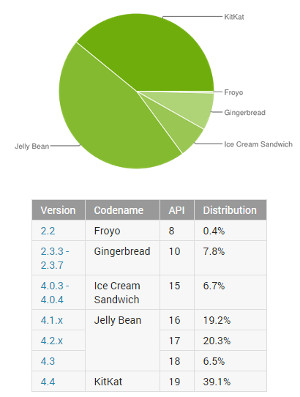
\includegraphics[scale=0.27]{android-versions}
	\caption{distributie van de Android versies in het begin van 2015}
	\label{fig:android_versions}
\end{figure}

\section{Batterijgebruik en efficiëntie}
Momenteel verbruikt de Android applicatie veel energie omdat continu gegevens opgevraagd worden over het netwerk. Ook de locatie van de gebruiker wordt frequent opgevraagd.
Een oplossing voor dit probleem is o.a. caching van gegevens en geofencing. Wanneer een gebruiker informatie opvraagt kan een lokaal opgeslagen versie van het resultaat getoond worden. In 1 oproep naar de backend kan gecontroleerd worden of nieuwe informatie voor handen is. Indien dit het geval is, kunnen de laatste gegevens binnengehaald worden van de servers. Deze oplossing wordt reeds toegepast op informatie over locatie- en overzichtelementen. Als cache of lokale databank wordt een SQLite database gebruikt. Dit systeem wordt aangeboden door Android. Caching van alle data zoals de oplossing voorstelt is nog niet geïmplementeerd wegens het beperkte tijdskader van het vakoverschrijdend project.
Geofencing is een manier voor locatiegebaseerde applicaties om te verhinderen dat continu locatiegegevens via GPS opgevraagd dienen te worden. Deze oplossing werd uitvoerig bestudeerd, maar kon wegens tijdsgebrek niet in de eindoplossing opgenomen worden.


